\section{Analysephase}

\subsection{Ist-Analyse}
Aktuell wird \Gls{Centreon} eingesetzt, soll jedoch in naher Zukunft durch \Gls{Checkmk} ersetzt werden.
Doch die Checks, welche für \Gls{Centreon} erstellt wurden, werden dann nicht mehr funktionieren.
Für \Gls{Checkmk} gibt es keine fertige Lösung, um eine Integration mit \Gls{MetricQ} zu ermöglichen.
Hier ist ein Ausschnitt eines solchen Checks:

\begin{lstlisting}[language=Python, caption=Centreon Check]
{
  "_id": "some_id",
  "_rev": "42",
  "$schema": "https://url.com/config.schema.json",
  "nsca": {
    "host": "some-address.de",
    ...
  },
  "overrides": { "ignored_metrics": ["just_a_test", "another_test"] },
  "nsca_backup": {
    "password": ...
  },
  "reporting_host": "--metricq--",
  "resend_interval": "3min",
  "checks": {
    "ColddoorTemperature": {
      "metrics": [
        "metric.1.something",
        "metric.2.something"
      ],
      "warning_above": 21,
      "critical_above": 42,
      "timeout": "420s"
      ],
    },
  }
...
}
\end{lstlisting}

\noindent
Wie hier zu sehen ist, muss sehr viel manuell erstellt und konfiguriert werden.
So muss z.\,B. die IP-Adresse des \Gls{Centreon}-Server angegeben werden.
Bei den checks müssen auch die Metriken angegeben werden.
Des Weiteren müssen sämtliche Schwellwerte angegeben werden.
Zusätzlich besteht hierbei nicht die Möglichkeit zu unterscheiden, ob eine Metrik nicht antwortet oder einen Wert außerhalb des erlaubten Spektrums hat, da dies in die Zuständigkeitsbereiche von verschiedenen Personen fällt.

\subsection{Soll-Analyse}\label{sec:soll-analyse}
Mit der neu entwickelten Anwendung soll neue Hardware mit minimalem Konfigurationsaufwand überwacht werden können.
Zudem sollen die Daten der Metriken wie bisher auch an das Monitoring übermitteln, mit dem Unterschied, dass sie diese nun nicht mehr an \Gls{Centreon} sendet, sondern für \Gls{Checkmk} bereitstellt.
Hier ist ein Überblick, wie der Code die Interaktion zwischen \Gls{MetricQ} und \Gls{Centreon} handhabt:

\begin{figure}[H]
  \centering
  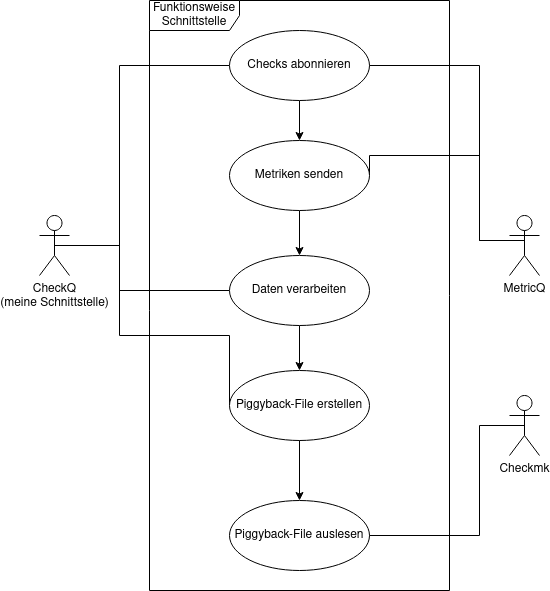
\includegraphics[height=0.5\textwidth]{images/use-case-checkq.png}
  \caption{Use Case der Schnittstelle}
\end{figure}

\noindent
Der Quellcode soll objektorientiert und modular aufgebaut sein. Dabei wird auf Wiederverwendbarkeit, Lesbarkeit sowie die Einhaltung gängiger Clean-Code-Prinzipien geachtet.
Tests sollen Funktionen, Codequalität und Datenstrukturen abdecken und gegebenenfalls genauere Informationen zur Behebung potenzieller Fehler liefern.
Der Kunde soll die Möglichkeit haben im Monitoring den derzeitigen Wert des Checks zu sehen.
In \Gls{Checkmk} hat jeder Check einen Status, welcher aussagt ob er in Ordnung ist oder nicht.
Ich habe hier eine Tabelle zusammengestellt, welche die verschiedenen Status bezeichnet:

\begin{table}[H]
  \centering
  \begin{tabular}{l l}
    \hline
    \textbf{Status} & \textbf{Bedeutung} \\
    \hline
    Ok     & Check ist in Ordnung \\
    WARN   & Check hat ein kleines Problem \\
    CRIT   & Check hat ein extremes Problem \\
    UNKNOWN & der Zustand des Checks ist nicht bekannt \\
  \end{tabular}
  \caption{Checkmk Check-Zustände}
\end{table}

\noindent
An den Code wurden durch den Kunden folgende weitere Anforderungen gestellt:

\begin{enumerate}
  \item Die Implementierung soll mittels einer von \Gls{MetricQ} unterstützten Sprache durchgeführt werden.
  \item Externe Bibliotheken sind auf Standardbibliotheken zu beschränken, mit den Kriterien, dass sie beim
    Programmieren unterstützen, weit verbreitet sind und aktuell gehalten werden.
  \item Der Programmcode soll mit modernen Programmiersprachen \Gls{feature} geschrieben werden.
\end{enumerate}

\subsection{Wirtschaftlichkeitsanalyse}

\subsubsection{Make or Buy-Entscheidung}
Es kann nur eine \texttt{Make}-Entscheidung getroffen werden, da das \Gls{framework} \Gls{MetricQ} eine hausinterne Entwicklung ist und nicht weit verbreitet ist.
Aufgrund dieser spezifischen Entwicklung ist es schwierig, ein fertiges Produkt zu erwerben.

\subsubsection{Projektkosten}
Die Berechnung der Projektkosten basiert auf den geschätzten Personal- und Ressourcenkosten.
Für die Kalkulation des Stundenlohns wurde der Bruttolohn eines Auszubildenden im dritten Lehrjahr gemäß Tarifvertrag der \acrshort{TU} Dresden herangezogen.
Dieser beträgt monatlich \qty{1190.61}{\euro} brutto\cite{TU_Dresden_Arbeiten}.

\noindent
Um den Stundenlohn zu ermitteln, wird der Bruttolohn für drei Monate durch die Arbeitszeit von 40 Stunden pro Woche über 13 Wochen geteilt:

\[
  \frac{3 \cdot 1190,61 \, \text{€}}{13 \cdot 40 \, \text{h}} \approx 6,87 \, \frac{\text{€}}{\text{h}}
\]

\noindent
Der berechnete Stundenlohn von \qty{6,87}{\euro} wurde zur Vereinfachung auf \qty{7}{\euro} aufgerundet.
Zusätzlich zu den Personalkosten fallen Ressourcenkosten für Räumlichkeiten, Software, Hardware und andere Betriebsmittel an.
Diese wurden pauschal mit einem Stundensatz von \qty{20}{\euro} angesetzt, basierend auf internen Rückmeldungen von Kollegen.

\noindent
Für den Auftraggeber wurde ein Stundensatz von \qty{27}{\euro} angenommen.
Dieser Wert orientiert sich an branchenüblichen Gehältern, die über die Plattform Stepstone\cite{informatiker-gehalt-lit} recherchiert wurden.
Bei der Entwicklung des Projekts wird mich ein Kollege bei spezifischen Fragen zu \Gls{Checkmk} unterstützen.
Für ihn wurde ebenfalls ein Stundensatz von \qty{27}{\euro} angesetzt.

\noindent
Die Gesamtkosten des Projekts belaufen sich auf \qty{2854}{\euro}.
Eine detaillierte Aufschlüsselung der Kosten ist in \reference{tab:kostenrechnung} dargestellt.

\begin{table}[H]
  \centering
  \small  % kleinere Schrift
  \renewcommand{\arraystretch}{1.1}  % geringerer Zeilenabstand
  \begin{tabular}{
      >{\raggedright\arraybackslash}p{5.2cm}
      >{\centering\arraybackslash}p{2.2cm}
      >{\raggedright\arraybackslash}p{5.5cm}
      >{\centering\arraybackslash}p{2.4cm}
    }
    \toprule
    \textbf{Tätigkeit} & \textbf{Dauer [h]} & \textbf{Stundensätze} & \textbf{Gesamt [€]} \\
    \midrule
    Projektbearbeitung
    & 80
    & \SI{7}{\euro} (Pers.) + \SI{20}{\euro} (Ress.)
    & \num{2160} \\

    Teammeetings
    & 7
    & 2 × \SI{27}{\euro} + \SI{20}{\euro}
    & \num{518} \\

    Fachliche Abstimmung
    & 5
    & \SI{7}{\euro} + 3 × \SI{27}{\euro} + \SI{20}{\euro}
    & \num{540} \\
    \midrule
    \multicolumn{3}{r}{\textbf{Gesamtkosten:}} & \textbf{\num{3218}} \\
    \bottomrule
  \end{tabular}
  \caption{Projektkosten – kompakte Übersicht}
  \label{tab:projektkosten}
\end{table}

\subsubsection{Amortisationsdauer}
In diesem Abschnitt wird ermittelt, ab welchen Zeitpunkt die \Gls{amortisierung} erfolgt ist, d.\,h. ab welchen Punkt die Kosten für das Projekt wieder eingenommen wurden.
Durch diesen Wert lässt sich eine Aussage treffen, ob die Umsetzung aus wirtschaftlicher Sicht angemessen ist und ob sich auf Dauer, Kostenvorteile ergeben können.
Durch die Entwicklung dieser Schnittstelle kann weiterhin sichergestellt werden, dass Probleme im Rechenzentrum frühzeitig erkannt werden.
Somit können sich Defekte sich nicht auf andere Komponenten ausbreiten können, oder auch Ausfälle schnell beseitigt werden können, bevor sich die Auswirkungen auf den Endnutzer bemerkbar machen
Wenn z.\,B. die Kühlung von einem \Gls{node} innerhalb eines \Gls{rack} fehlschlägt, kann dies schnell zu Problemen führen.
Es könnte beispielsweise eine \acrshort{CPU}s\cite{cpu-lit} fehlen, welche dann sofort ausfallen, was einen großen Schaden wäre.

\noindent
Im aktuellen Hochleistungsrechner der \acrshort{TU} Dresden, gibt es pro \Gls{node} 2 \Gls{socket}s, mit je einem \textbf{Intel(R) Xeon(R) Platinum 8470} als \acrshort{CPU}.
Den Preis habe ich laut der Intel Webseite\cite{intel-xeon-lit} auf \qty{9359.00}{\$} pro \acrshort{CPU} bestimmt.
Daraus habe ich folgende Rechnung gemacht.
Ich habe angenommen, dass durch einen Ausfall der Kühlung und zu spätes Handeln 5 \Gls{node}s kaputtgehen, in dem die \acrshort{CPU}s überhitzen.

\noindent
Hier habe ich die \acrshort{CPU} Kosten pro \Gls{node} ausgerechnet.
\[
  \qty{9359.00}{\USD} \times 2 = \qty{18718.00}{\USD}
\]

\noindent
Die \qty{18718.00}{\USD} habe ich dann mit den 5 \Gls{node}s multipliziert.

\[
  \qty{18718.00}{\USD} \times 5 = \qty{93590.00}{\USD}
\]

\noindent
Die Kosten betragen somit ca. \qty[group-separator={.}]{93590}{\USD}, was umgerechnet etwa \qty[group-separator={.}]{86000}{\euro} entspricht (Stand 2024, Wechselkurs ca. 1,\$ = 0,92,€).
Schon das Verhindern eines einzigen Node-Ausfalls amortisiert die Projektkosten mehrfach.

\subsection{Anwendungsfälle}
Ein typischer \Gls{anwendungsfall} ist ein Kühlungsausfall im Rechenzentrum.
In dem Fall würden in \Gls{MetricQ} die Temperaturwerte der \Gls{node}s, sowie die \Gls{socket}s gelesen werden.
Diese steigen kontinuierlich an, bis die definierten Schwellwerte erreicht werden.
Wenn die Schwellwerte erreicht sind, werden automatisiert Benachrichtigungen durch das Monitoring an die zuständigen Personen geschickt.
Dies habe ich auch als \acrlong{EPK} (\acrshort{EPK}) abgebildet, dieses ist im Anhang \reference{fig:epk-cooling-fails} zu finden.
Ein weiterer Anwendungsfall ist die automatische Erkennung von Änderungen in der Struktur, z.\,B. wenn ein neues Rack hinzugefügt wurde.
Zuerst werden die neuen Metriken zu \Gls{MetricQ} hinzugefügt und die Schnittstelle neu konfiguriert.
Die Dienstanwendung würde dann die Änderungen erkennen, in dem es neue Metriken gibt.
Für diese Metriken würden dann neue Checks generiert werden.
Durch die automatische Generierung von Checks entfällt der manuelle Konfigurationsaufwand vollständig.
Diese würden dann wie bei den bisherigen Checks ihre Überprüfungen machen und diese an das Monitoring weiterleiten.
Hierzu habe ich ebenfalls ein \acrlong{EPK} abgebildet, dieses ist im Anhang \reference{fig:epk-structure-changes} zu finden.

\subsection{Qualitätsanforderungen}\label{sec:qualitätsanforderungen}
An die Anwendung wurden mehrere Qualitätssicherungsanforderungen gestellt.
Es ist erforderlich, dass beim Programmieren moderne Features verwendet werden, die die Effizienz und Wartbarkeit des Codes verbessern.
Der Code soll einheitlich, gut dokumentiert und leicht nachvollziehbar sein.
Jeder Anwendungsfall sollte eindeutig beschrieben werden, um Missverständnisse zu vermeiden und die Anforderungen klar zu definieren.
Der Code ist in objektorientierter Programmierung zu verfassen, was die Modularität und Wiederverwendbarkeit erhöht.
Darüber hinaus sollte der Entwicklungsprozess möglichst automatisiert gestaltet werden, um menschliche Fehler zu minimieren und die Effizienz zu steigern.
Schließlich ist es wichtig, dass die Anwendung durch Unit-Tests umfassend getestet wird, um die Zuverlässigkeit und Funktionalität der Software sicherzustellen.
Für Unit-Tests wird \texttt{pytest} eingesetzt. Die Einhaltung von Codekonventionen wird mittels \texttt{flake8} und \texttt{black} sichergestellt.
